\chapter{Generalize F-TRACT approach to TMS-EEG}\label{ch:pytepfit}

The main goal of this thesis is to apply the approach by Seguin et al. \cite{seguin_communication_2023} rooted in complex network analysis and compare its applicability in empirical and simulated EEG recordings of TMS evoked potentials. As explained in Section \ref{sec:tms-eeg_measurement}, the TMS-EEG measurement is indirect; it does not require the implantation of electrodes in the brain. Because of that, it is easier to use it in research, but it is less precise. We want to see if it is possible to get an insight into the response structure using the communication models for TMS-EEG data similarly as it was presented in Sections \ref{sec:ftract_results} and \ref{sec:ftract_results_per_roi} for iEEG data. 

\section{TMS-EEG data}\label{sec:reponse_definition}

There are several key differences between the summarized iEEG functional data available in F-TRACT and the TMS-EEG data used in this section. 

The F-TRACT dataset provides probabilities. For each ROI, there is a vector of probabilities that there are significant responses in the other ROIs aggregated on a group level. On the other hand, the TMS-EEG data used here are time series of a single subject capturing the time-resolved response for each ROI after the target site stimulation. another difference is that the TMS-EEG data in the dataset used in this thesis were measured with stimulation on a single site, while F-TRACT includes stimulations in many different sites.

Besides empirical data, we work with simulated TMS-EEG data, and we compare the results. This comparison may be useful as guidance for the future development of models for a generation of artificial TMS-evoked responses.

\subsection{Empirical data}

We used TMS-EEG data published by the Rogasch group\footnote{\url{https://figshare.com/articles/dataset/TEPs-_SEPs/7440713}} \cite{biabani_characterizing_2019} where high-density EEG was recorded following M1 stimulation in 20 healthy young individuals. TMS-EEG evoked potential (TEP) source reconstruction was performed by Momi et al. \cite{momi_tms-evoked_2023}, resulting in group-averaged time series, one time series per ROI in Schaefer200 parcellation (\ref{parc:Schaefer200}). See Figure \ref{fig:tms-empirical-data}. 

\begin{figure}
    \centering
    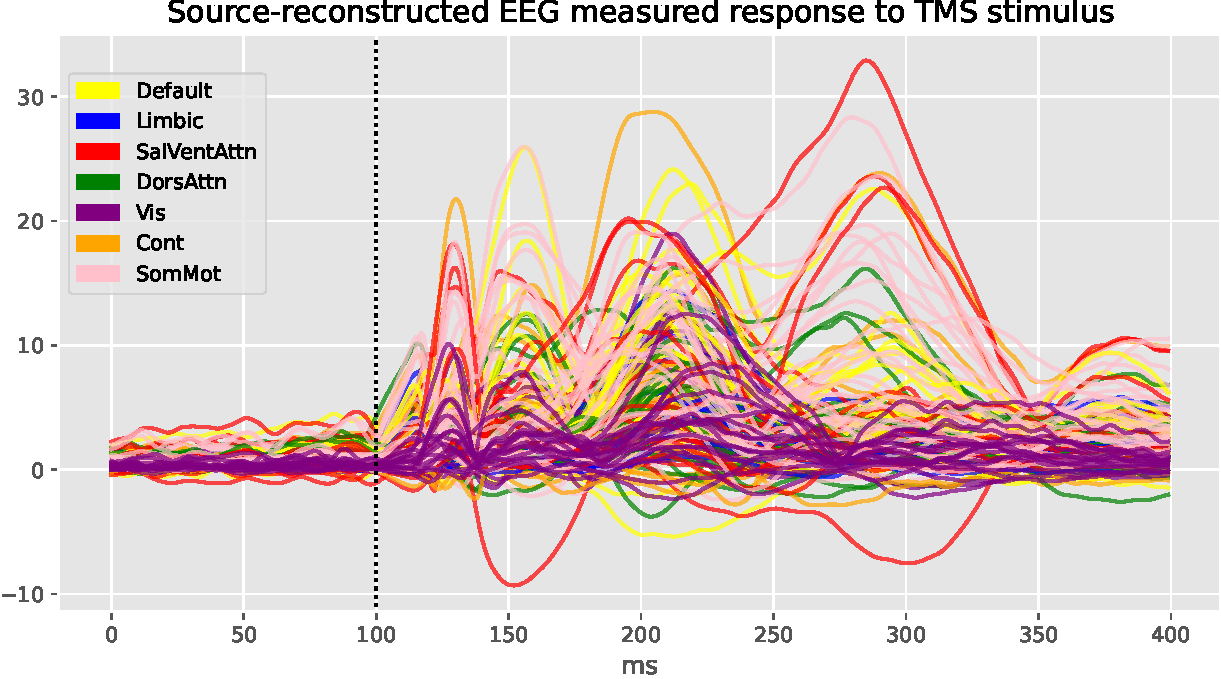
\includegraphics[width=\textwidth]{images/nootebook_generated/pytepfit_results/empirical/200/not_over_threshold_nan/data.pdf}
    \caption[TMS-EEG empirical data]{TMS-EEG empirical data, stimulation at 100 ms after the start of the measurement. The TEPs are colored based on Yeo7 (\ref{parc:Yeo}) functional networks. EEG source reconstructed, baseline corrected, and $z$-scored.}
    \label{fig:tms-empirical-data}
\end{figure}

\subsection{Simulated data}

Besides the source-reconstructed empirical TEPs, Momi et al. published simulated TEPs. The whole modeling process is described in their paper \textit{TMS-evoked responses are driven by recurrent large-scale network dynamics} \cite{momi_tms-evoked_2023}. 

Briefly, the model consists of 200 brain regions (based on Schaefer200 parcellation) connected by weights of an anatomical connectivity matrix. The nodes represent the averaged activity of the specific brain region and the activity in each node is modeled using a set of equations. \cite{deco_perturbation_2018} Then, the model was fitted to the empirical data of each subject, and the resulting TEPs were averaged. \cite{momi_tms-evoked_2023}

The resulting simulated data are plotted in Figure \ref{fig:tms-simulated-data}. We see that the TEPs are much smoother than the empirical in Figure \ref{fig:tms-empirical-data}.

\begin{figure}
    \centering
    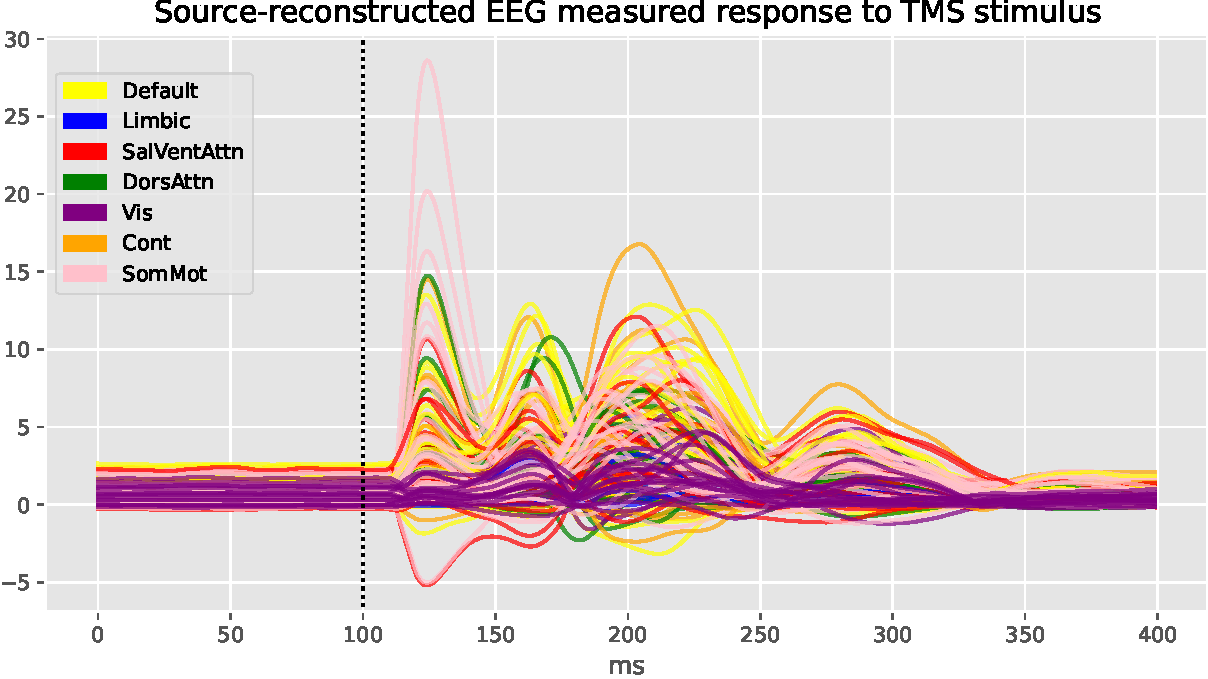
\includegraphics[width=\textwidth]{images/nootebook_generated/pytepfit_results/simulated/200/not_over_threshold_nan/data.pdf}
    \caption[TMS-EEG simulated data]{TMS-EEG simulated data, stimulation at 100 ms after the start of the measurement. The TEPs are colored based on Yeo7 functional networks. EEG source reconstructed, baseline corrected, and $z$-scored.}
    \label{fig:tms-simulated-data}
\end{figure}

\subsection{Quantification of TMS-EEG response}

To follow the methodology used by Seugin et al. for the F-TRACT data, it is necessary to decide how to quantify the time series of each ROI and, followingly, create a vector characterizing the response in the whole brain. We can not use the probability of the response because the TEPs were measured only in 20 subjects and we have the group-averaged data.

This section discusses all the options used later in the work. They are also visualized in Figure \ref{fig:tms-respondse-definition}.

\begin{itemize}
    \item \textbf{binary (01) response} If the TEP exceeds a predefined threshold, the value is set to 1, otherwise it is set to 0.
    \item \textbf{first/highest peak} The weight of the response is defined as the height of the first/highest peak above a predefined threshold. If the TEP does not exceed the threshold, it is set to \texttt{nan} and is not considered in the analysis.\footnote{Alternatively, we can replace all \texttt{nan}s in the definitions with zeros and include them in the analysis. The approaches capture different properties of the response.} The highest peak corresponds to amplitude in F-TRACT. 
    \item \textbf{first/highest peak latency} The weight of the response is defined as the latency of the the first/highest peak above a predefined threshold occurs. If the TEP does not exceed the threshold, it is set to \texttt{nan} and is not considered in the analysis. The idea behind this definition is that we assume the response to propagate faster to regions that are \uv{more} connected (for example, there are edges with higher weights or shorter lengths in structural connectome).
    \item \textbf{AUC} The weight of the response is defined as the area under the curve if the curve exceeds a predefined threshold, \texttt{nan} otherwise. The key idea of this definition is that AUC captures the overall \uv{power} of the response. It is systematically different from the other definitions, so it might reveal different relationships.
\end{itemize}

We considered also variance, mean, difference of the lowest and the highest value, AUC of the area above the threshold, etc., but we did not include them because they are very similar to the ones in the list.

\begin{figure}
    \centering
    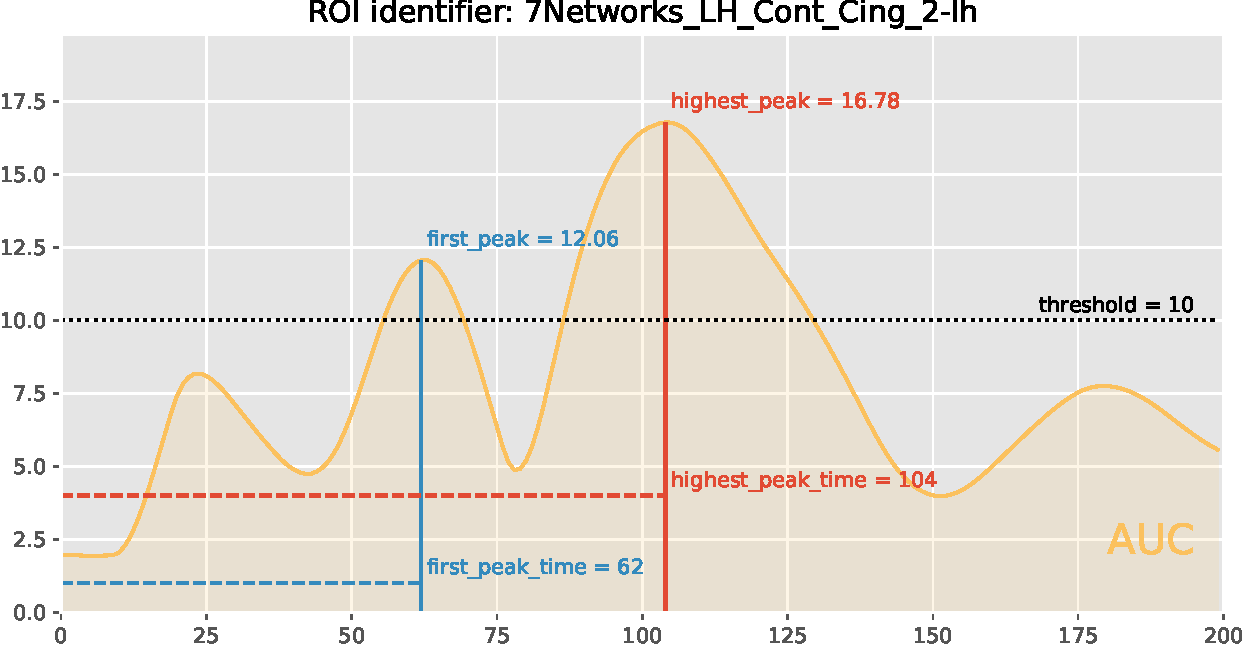
\includegraphics[width=\textwidth]{images/nootebook_generated/pytepfit_results/simulated/200/not_over_threshold_nan/7Networks_LH_Cont_Cing_2-lh_response_def.pdf}
    \caption[TMS-EEG response definitions -- illustration]{Definitions of the quantification of TMS-EEG response - illustration with one ROI, 200 ms response (stimulus at 0). EEG source reconstructed, baseline corrected, and $z$-scored.}
    \label{fig:tms-respondse-definition}
\end{figure}

\subsubsection{Threshold selection}

All the response definitions work with some threshold. There is always a baseline activity in the brain, as shown in Figure \ref{fig:tms-empirical-data} before the stimulation. We need to filter out the activity after the stimulation caused by this natural process and keep only responses truly evoked by the TMS stimulation. However, there is nothing like \uv{the right threshold} and it depends on the specific data used in each case. Because of that, we tried several thresholds, the lowest corresponding to the highest peak in the activity before the stimulation and the highest selected such that there are at least 30 TEPs over that threshold to keep enough data for statistics.

\subsubsection{Response length}

Besides the threshold, it is important to select the length of the response we want to consider. The later responses can be confounded by the auditory stimulus (loud TMS click), and somatosensory responses i.e., activation of cranial nerves). \cite{hernandez-pavon_tms_2023} On the other hand, as shown in Section \ref{sec:response-length_F-Tract}, the earlier responses might be driven simply by the Euclidean distance. We tried several response lengths, including 50 ms and 200 ms, which gave us results comparable to those obtained using F-TRACT.

\section{Results for empirical data}\label{sec:results_pytepfit-empirical}

In this section, we present the results showing that, for some of the response definitions (specifically binarized TEP, AUC, and first peak height), there are significant correlations across various thresholds between the response and structural connectivity and the communication metrics derived from it. 

For the structural connectivity, we used the Mica-Mics dataset with Rosen and Halgrens's preprocessing method because it gave us the best results for the F-TRACT dataset (Section \ref{sec:sc-robustness_ftract}) and it also provides the Schaefer200 parcellation used here, which allows better comparison of the results. We used the Spearman correlation coefficient, results are considered significant for $p<0.05$.

\subsection{Binarized response}

First, if the response is binarized, it correlates with Euclidean distance across response lengths 50, 100, 150, 200, and 300 milliseconds and various thresholds ($r \approx 0.4$ depending on the parameters). It serves as an assurance that the calculations are correct because Sections \ref{sec:ftract_results} and \ref{sec:ftract_results_per_roi} show that there is a high correlation between the response probability and amplitude and Euclidean distance. 

We show the results for 200 ms response across various thresholds in Figure \ref{fig:tms_01_200}. The shortest path efficiency and navigation efficiency correlations are similar to those achieved with Euclidean distance, similar to the F-TRACT results in Figure \ref{fig:ftract_alldata_long_probabilities}.

\begin{figure}
    \centering
    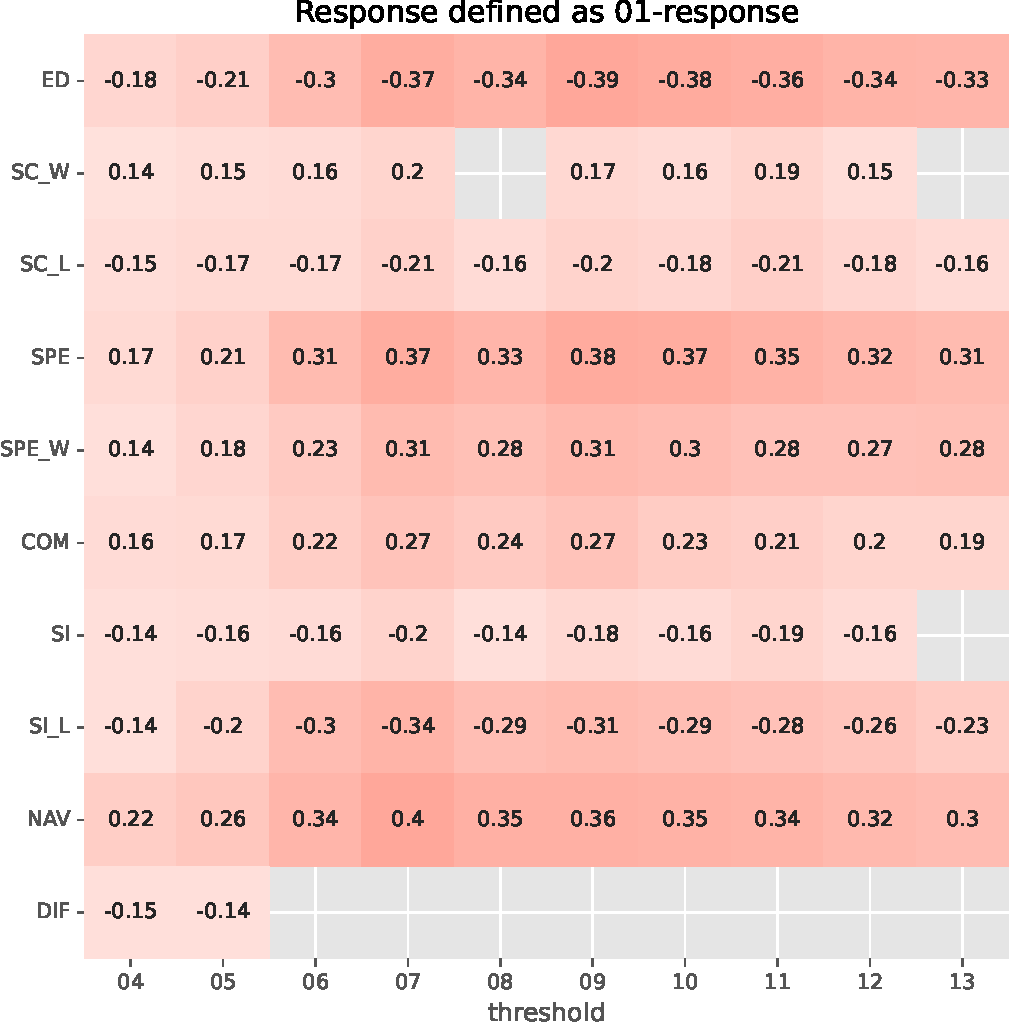
\includegraphics[width=\textwidth]{images/nootebook_generated/pytepfit_results/empirical/200/not_over_threshold_nan/Response defined as 01-response.pdf}
    \caption[Binarized TEP (200 ms) correlations]{Spearman correlation coefficient of binarized empirical TEP (200 ms response) with structural connectivity and communication metrics. Darker color denoted a higher absolute value of the correlation; missing values are non-significant ($p>0.05$).}
    \label{fig:tms_01_200}
\end{figure}

\subsection{Response characterized by AUC}

Based on our results, the AUC of TEP above a threshold correlates best with the structural connectivity and communication metrics.

The results for 50 ms response length (Figure \ref{fig:tms_auc_50}) differ from longer responses ($\geq100$ ms) because there are significant correlations consistently expressed only for Euclidean distance, shortest path efficiency, and navigation efficiency (and only for lower thresholds). For the longer responses (represented by Figure \ref{fig:tms_auc_200} for 200 ms), the correlations are overall higher and appear across various thresholds. 

Nevertheless, the response AUC correlation is consistently highest with Euclidean distance, the shortest path efficiency and navigation efficiency, followed by structural connectivity lengths, search information and communicability, which corresponds to the results in F-TRACT considering all pairs of ROIs (Figure \ref{fig:ftract_mica_short_probabilities} for 50 ms response and Figure \ref{fig:ftract_mica_long_probabilities} for 200 ms response).

\begin{figure}
    \centering
    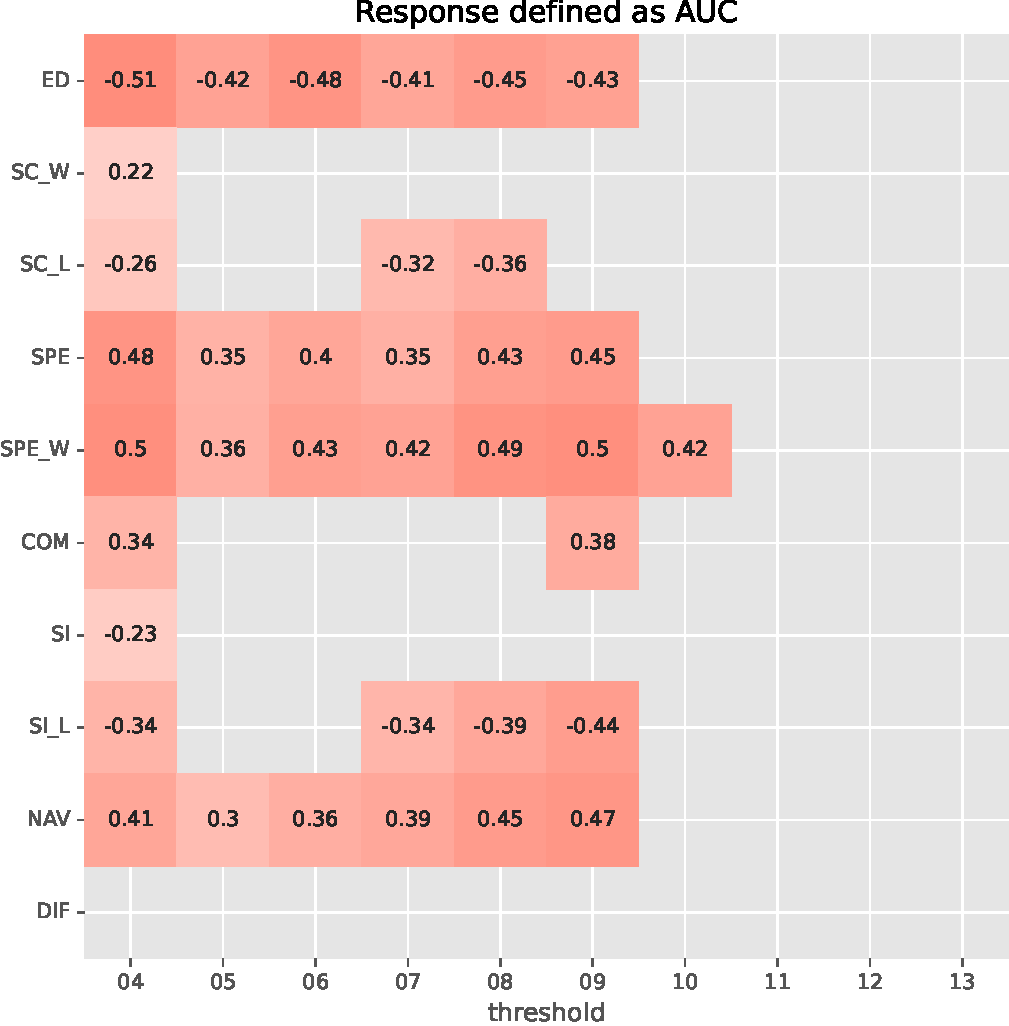
\includegraphics[width=\textwidth]{images/nootebook_generated/pytepfit_results/empirical/50/not_over_threshold_nan/Response defined as AUC.pdf}
    \caption[TEPs AUC (50 ms) correlation with SC and communication metrics]{Spearman correlation coefficient of AUC of empirical TEP (50 ms response) with structural connectivity and communication metrics. Darker color denoted a higher absolute value of the correlation; missing values are non-significant ($p>0.05$).}
    \label{fig:tms_auc_50}
\end{figure}

\begin{figure}
    \centering
    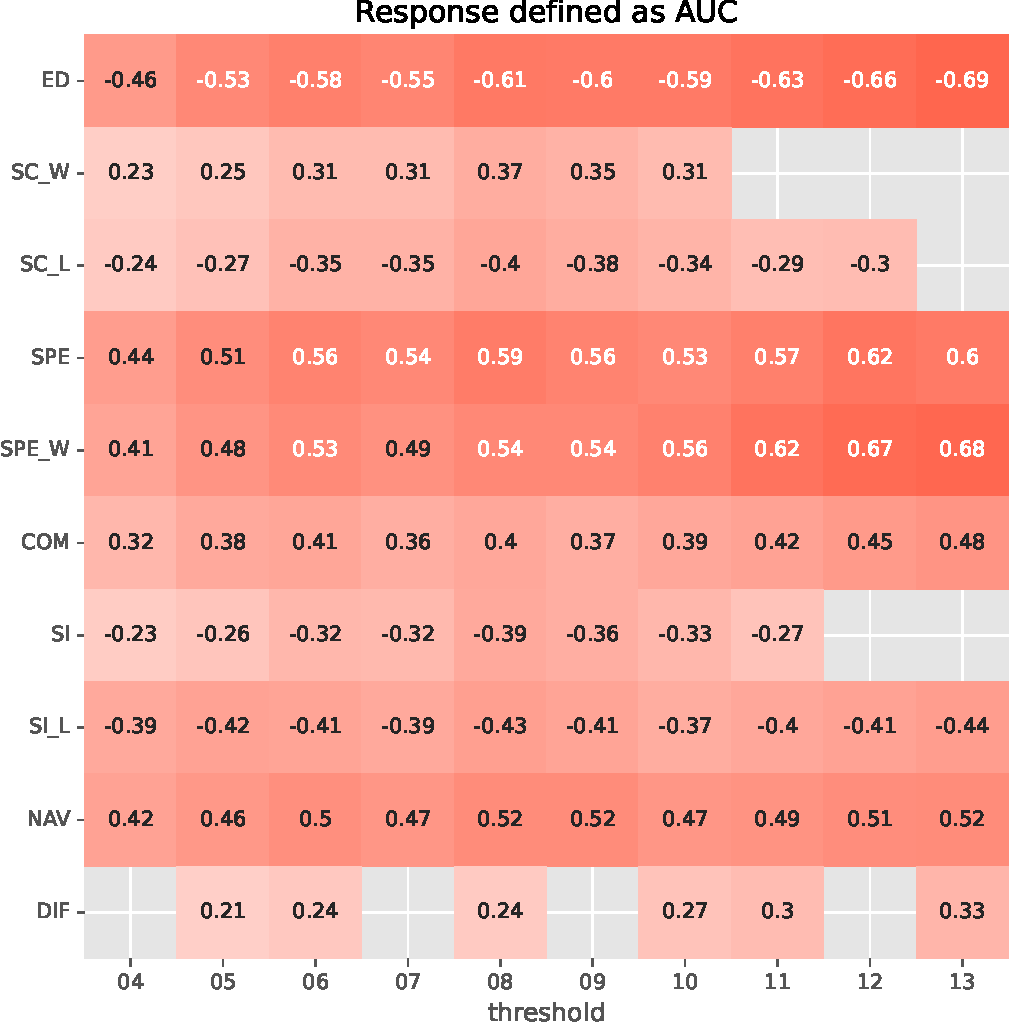
\includegraphics[width=\textwidth]{images/nootebook_generated/pytepfit_results/empirical/200/not_over_threshold_nan/Response defined as AUC.pdf}
    \caption[TEPs AUC (200 ms) correlations]{Spearman correlation coefficient of AUC of empirical TEP (200 ms response) with structural connectivity and communication metrics. Darker color denoted a higher absolute value of the correlation; missing values are non-significant ($p>0.05$).}
    \label{fig:tms_auc_200}
\end{figure}

\subsection{Response characterized by peak latencies}

If we characterize the response by the amount of time from the stimulation to the first peak, we need to consider an interval long enough so the peaks can occur. Looking at Figure \ref{fig:tms-empirical-data}, it could be seen that 50 ms is insufficient. Based on our experiments, we should take at least 150 ms response. 

Taking into account only responses longer than 150 ms, the first peak latency correlates with Euclidean distance, shortest path efficiency, navigation efficiency, and communicability across all the thresholds. See Figure \ref{fig:tms_first_time_200} for 200 ms response.

\begin{figure}
    \centering
    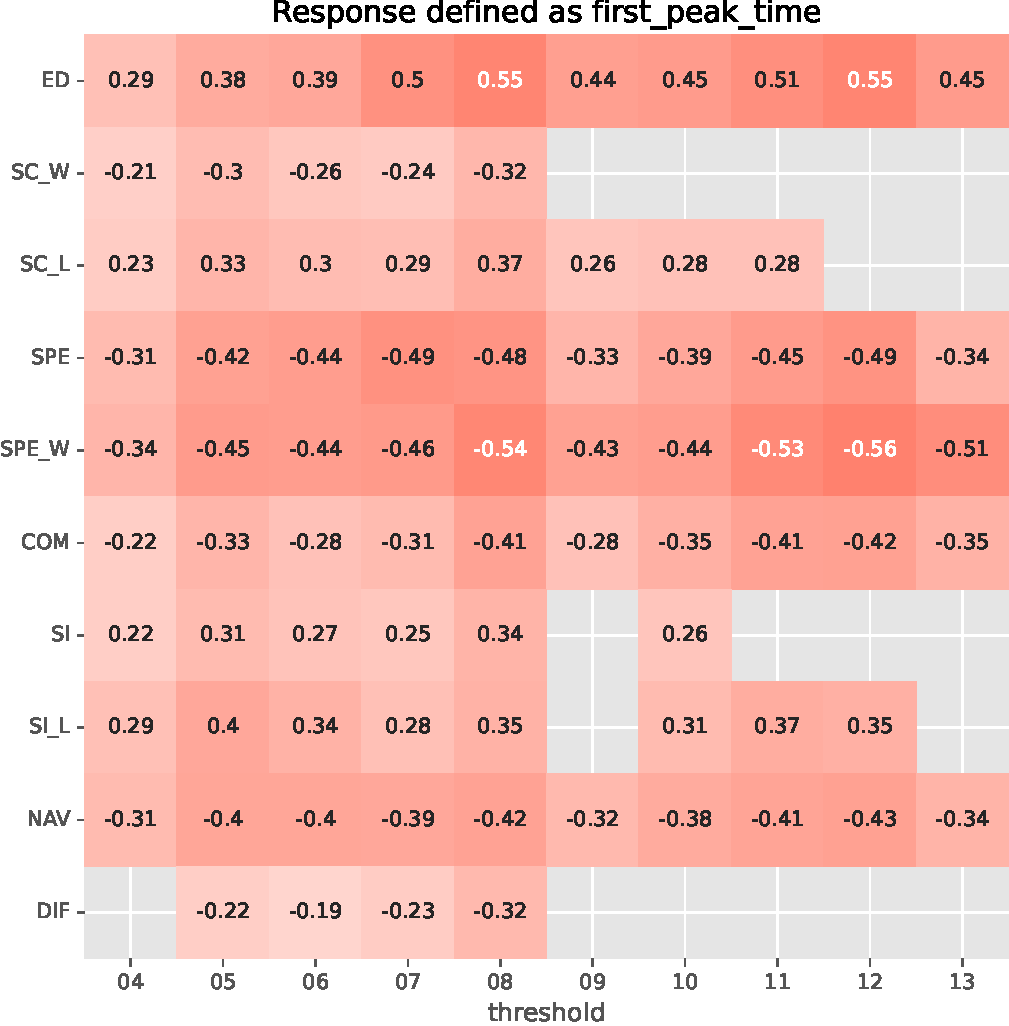
\includegraphics[width=\textwidth]{images/nootebook_generated/pytepfit_results/empirical/200/not_over_threshold_nan/Response defined as first_peak_time.pdf}
    \caption[TEPs first peak latency (200 ms) correlations]{Spearman correlation coefficient of the first peak latency in empirical TEP (200 ms response) with structural connectivity and communication metrics. Darker color denoted a higher absolute value of the correlation; missing values are non-significant ($p>0.05$).}
    \label{fig:tms_first_time_200}
\end{figure}

Characterizing the response by the highest peak latency proved to be a dead end, as the results are largely non-significant. There is an exception for a response length of 150 ms, which shows many significant correlations. It is probably because the highest peaks correspond to the first peaks for this response length; the plot for this setting looks very similar to the first peak latency responses shown in Figure \ref{fig:tms_first_200}. 

\subsection{Response characterized by peak heights}

Surprisingly, there are only a few significant correlations, only for lower thresholds, across all the response lengths when we use the highest peak as a response characterization. It seems that the relationship between the highest peak height and structural connectivity is weak, if any. It stands in contrast with the results obtained for response amplitudes from F-TRACT in Figure \ref{fig:ftract_alldata_long_amplitudes}, where we see significant correlations of the amplitudes with structural connectivity and communication metrics. See Figure \ref{fig:tms_heighest_200} for 200 ms response.

The height of the first peak does not exhibit any correlations with structural connectivity and communication metrics at all. 

\begin{figure}
    \centering
    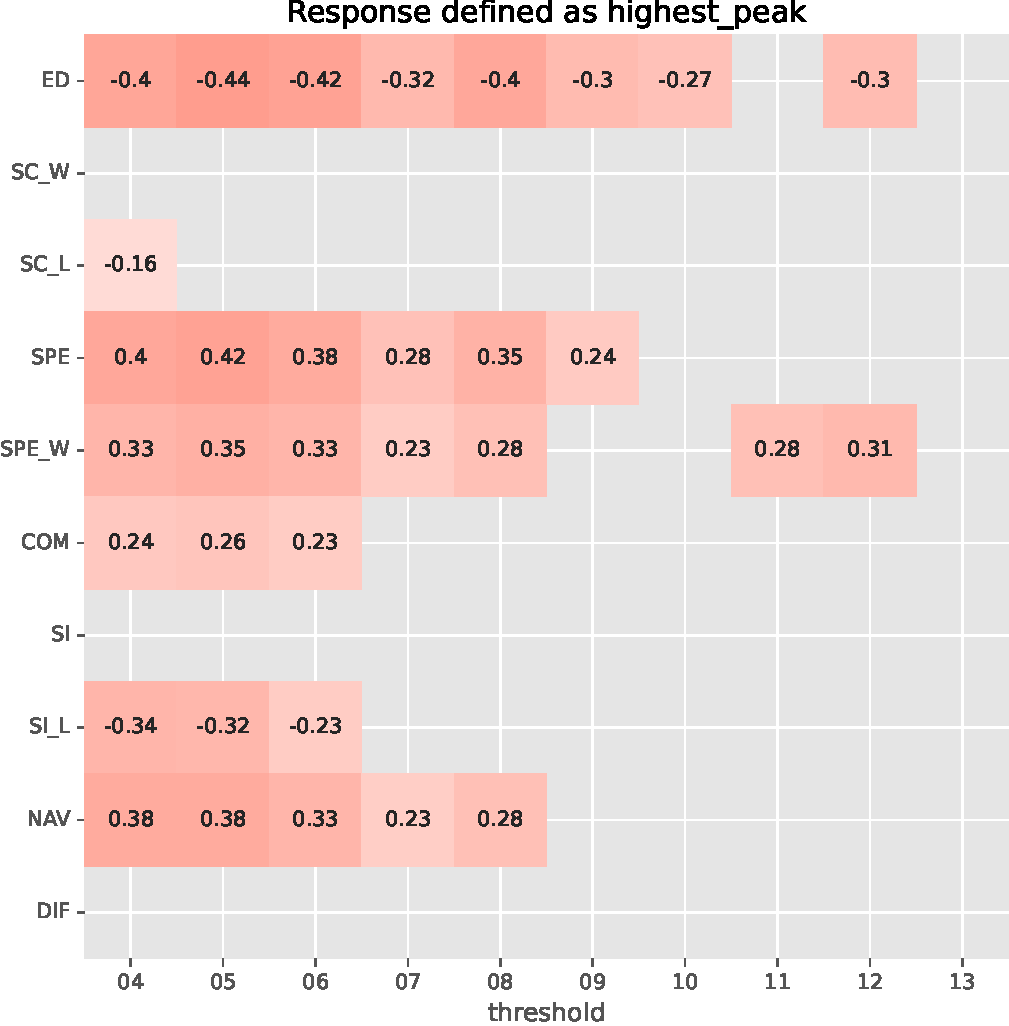
\includegraphics[width=\textwidth]{images/nootebook_generated/pytepfit_results/empirical/200/not_over_threshold_nan/Response defined as highest_peak.pdf}
    \caption[TEPs highest peak (200 ms) correlations]{Spearman correlation coefficient of the height of the highest peak in empirical TEP (200 ms response) with structural connectivity and communication metrics. Darker color denoted a higher absolute value of the correlation; missing values are non-significant ($p>0.05$).}
    \label{fig:tms_heighest_200}
\end{figure}

\subsection{Response length}

The results change with response length. As mentioned above, if the response is characterized by the first peak latency, the length should be at least around 150 ms. If the response is shorter, not all peaks occur in the time. 

If we characterize the response using AUC, the results for a really short response length (50 ms) are different from the other response lengths ($\geq100$ ms), as shown in Figure \ref{fig:tms_auc_50} and Figure \ref{fig:tms_auc_200}.

\section{Empirical vs simulated data}

The main question we aim to answer by comparing results for empirical and simulated data is if the simulated data express similar behavior to the empirical ones. We can see just by looking at Figures \ref{fig:tms-empirical-data} and \ref{fig:tms-simulated-data} that the distribution, height, and timing of the peaks and AUC are different. 

Does it mean that the data act differently concerning the analysis of the response correlation with structural connectivity and communication metrics? The possible similarity of the results could mean that the simulated data grasps some aspects of the empirical data and we can study the simulated data to reveal some aspects of the nature of the brain.

\subsection{Similarities}

The first important similarity lies in the results for the binarized response. It shows the same pattern as we have seen before, the response correlates with Euclidean distance, the shortest path efficiency, and the navigation efficiency. Figure \ref{fig:tms_binary_100_simulated} shows that for 100 ms response. 

\begin{figure}
    \centering
    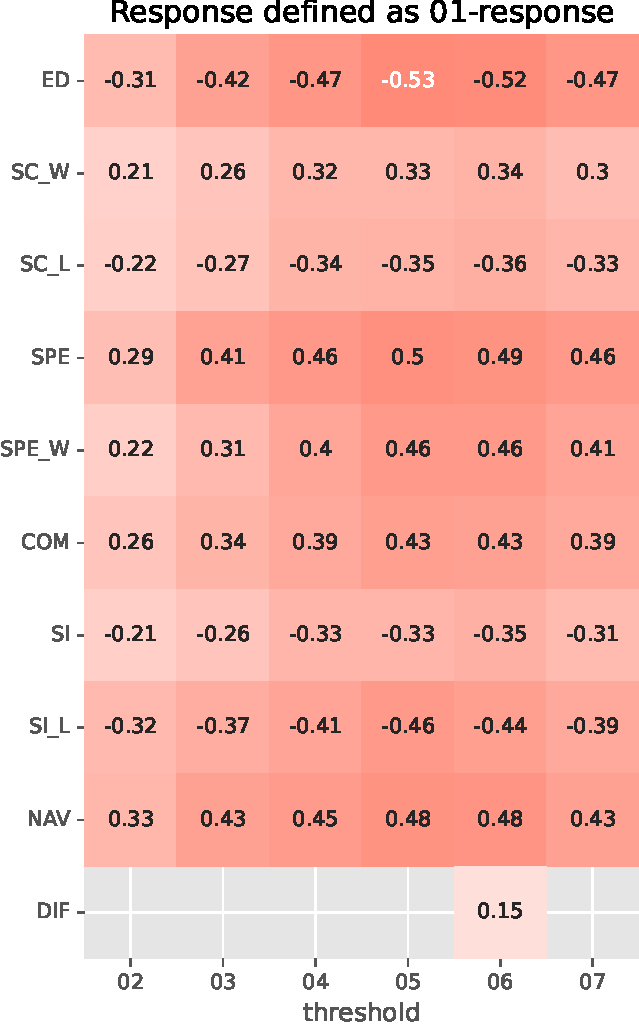
\includegraphics[height=\textwidth]{images/nootebook_generated/pytepfit_results/simulated/100/not_over_threshold_nan/Response defined as 01-response.pdf}
    \caption[Binarized TEP (100 ms) correlations (simulated data)]{Spearman correlation coefficient of binarized empirical TEP (100 ms response) with structural connectivity and communication metrics. Darker color denoted a higher absolute value of the correlation; missing values are non-significant ($p>0.05$).}
    \label{fig:tms_binary_100_simulated}
\end{figure}

Another similarity can be found in the response characterized by the first peak latency. Even though the correlations are overall higher for simulated data, Figure \ref{fig:tms_first_time_200_simulated} shows a similar pattern to Figure \ref{fig:tms_first_time_200} with the highest correlations of the first peak latency with Euclidean distance, shortest path efficiency and navigation efficiency across all thresholds. 

\begin{figure}
    \centering
    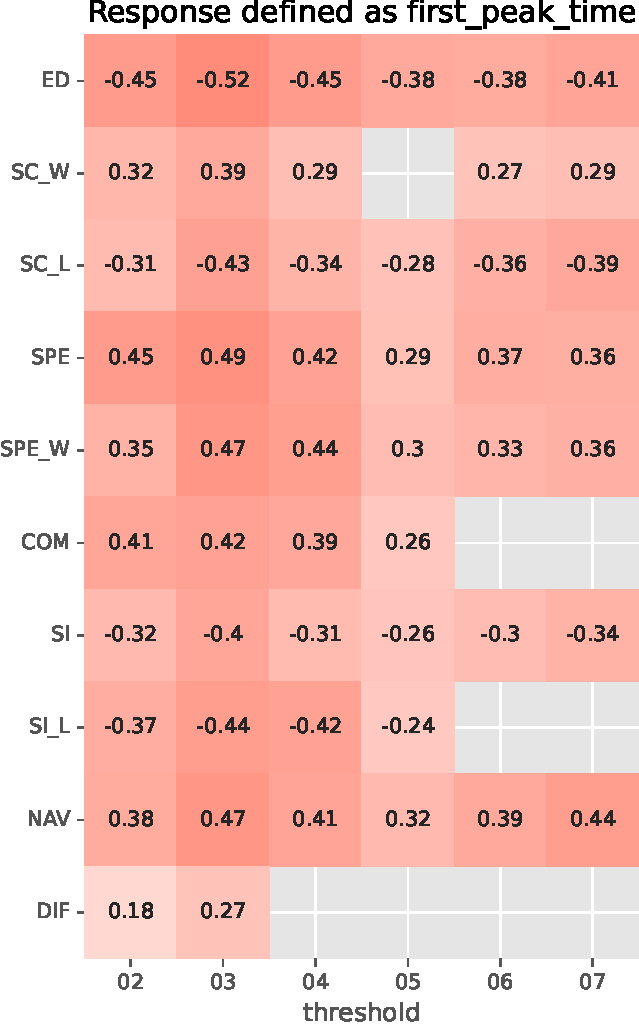
\includegraphics[height=\textwidth]{images/nootebook_generated/pytepfit_results/simulated/200/not_over_threshold_nan/Response defined as first_peak_time.pdf}
    \caption[TEPs first peak latency (200 ms) correlations (simulated data)]{Spearman correlation coefficient of the first peak latency in simulated TEP (200 ms response) with structural connectivity and communication metrics. Darker color denoted a higher absolute value of the correlation; missing values are non-significant ($p>0.05$).}
    \label{fig:tms_first_time_200_simulated}
\end{figure}

\subsection{Differences}

Unsurprisingly, there are many differences in the results calculated using simulated and empirical data. First of all, considering a response length of at least 100 ms, the highest correlations of the response with communication metrics are obtained for response strength defined as its highest peak latency (Figure \ref{fig:tms_highest_time_200_simulated} for 200 ms response).

\begin{figure}
    \centering
    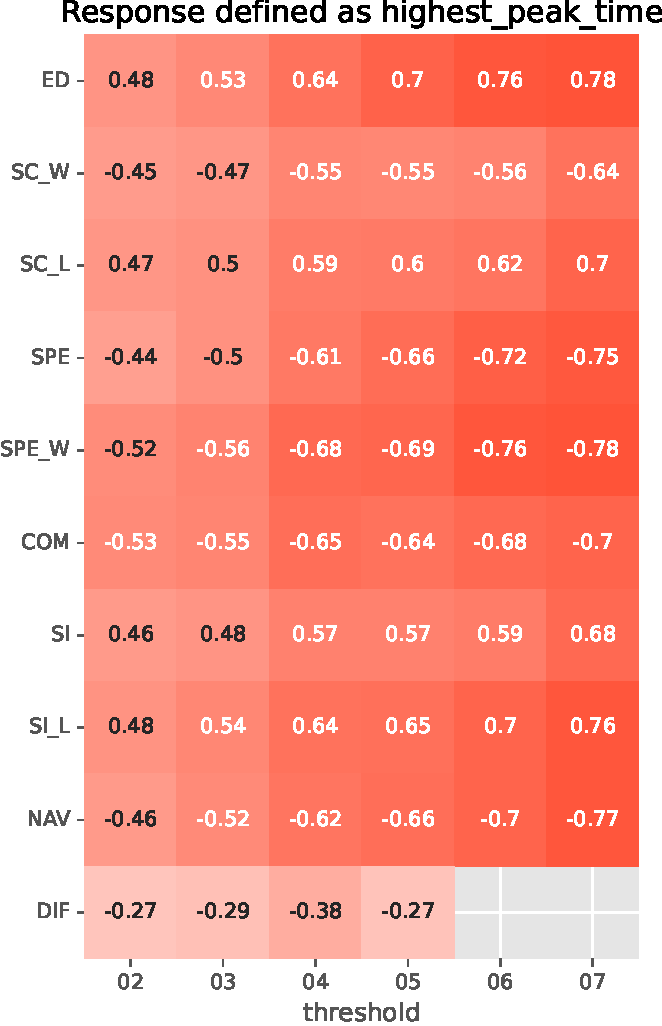
\includegraphics[height=\textwidth]{images/nootebook_generated/pytepfit_results/simulated/200/not_over_threshold_nan/Response defined as highest_peak_time.pdf}
    \caption[TEPs highest peak latency (200 ms) correlations (simulated data)]{Spearman correlation coefficient of the highest peak latency in simulated TEP (200 ms response) with structural connectivity and communication metrics. Darker color denoted a higher absolute value of the correlation; missing values are non-significant ($p>0.05$).}
    \label{fig:tms_highest_time_200_simulated}
\end{figure}

Response characterized by AUC correlates much worse with structural connectivity and communication metrics if it is calculated using the simulated data, as shown in Figure \ref{fig:tms_AUC_200_simulated}. On the other hand, the height of the peaks correlates better with communication metrics for the simulated data than for the empirical data (but worse than other response characteristics for simulated data). 

\begin{figure}
    \centering
    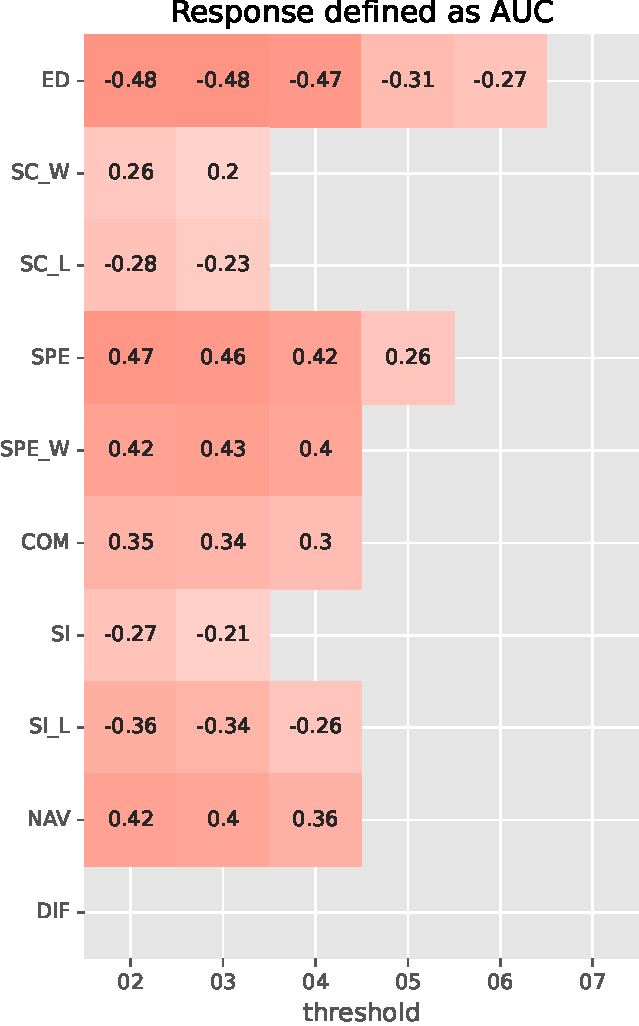
\includegraphics[height=\textwidth]{images/nootebook_generated/pytepfit_results/simulated/200/not_over_threshold_nan/Response defined as AUC.pdf}
    \caption[TEPs AUC (200 ms) correlations (simulated data)]{Spearman correlation coefficient of AUC of simulated empirical TEP (200 ms response) with structural connectivity and communication metrics. Darker color denoted a higher absolute value of the correlation; missing values are non-significant ($p>0.05$).}
    \label{fig:tms_AUC_200_simulated}
\end{figure}

In conclusion, the similarities and differences seem to follow the difference in data simulation and generation through the natural process in the brain. The simulated data capture the highest peak timings, which might be noisy in the empirical data. On the other hand, the simulated data probably do not model very well the overall complexity of the response, captured by AUC in the empirical data. 

The correlations with communication models are overall higher for simulated data. This might be because of the lower noise, but also because of the lack of more complex interactions in the modeled data. The model is a simplified description of the complex process, which might result in higher correlations with the simplified description of the communication using communication models. 

All the differences could be used for the next iteration of TMS-EEG simulating model development.